\section{Wyniki pomiarów działania programu}
\subsection{Dokładność modeli w bazie}
Badania przeprowadzono dla różnych liczb n-literowych końcówek wyrazów. Aby lepiej zobrazować otrzymane wyniki użyto notacji (\textit{liczba 1 literowych końcówek, liczba 2 literowych końcówek, liczba 3 literowych końcówek, liczba 4 literowych końcówek}).
\begin{landscape}
	\begin{table}[!htbp]
		\centering
		\caption{Skuteczność modeli -- Korpus PWr}
		\begin{tabular}{cccccccc}
			\hline
			\multicolumn{1}{|c|}{\textbf{Algorytm}} & \textbf{(15, 35, 35, 35)} & \textbf{(20, 35, 35, 35)} & \textbf{(25, 38, 38, 38)} & \textbf{(25, 40, 40, 40)} & \textbf{(28, 42, 42, 42)} & \textbf{(28, 45, 45, 45)} & \textbf{(32, 45, 45, 45)} \\ \hline
			Support Vector Machine & 56,46 & 57,46 & 58,75 & 60,03 & 61,01 & 59,94 & 58,68 \\
			Decision Trees & 57,24 & 58,12 & 59,30 & 59,97 & 60,58 & 59,10 & 58,14 \\
			Stochastic Gradient Descent & 53,62 & 54,48 & 55,37 & 56,58 & 57,72 & 56,22 & 54,97 \\
			Logistic Regression & 55,57 & 56,68 & 57,93 & 58,82 & 59,93 & 58,79 & 57,84 \\
			Naive Bayes & 54,14 & 55,42 & 56,69 & 57,72 & 58,89 & 57,58 & 56,56 \\
			K Neighbors & 50,17 & 51,35 & 52,18 & 53,30 & 54,22 & 53,12 & 52,20 \\
			Neural Networks & 55,80 & 57,08 & 57,91 & 58,88 & 60,04 & 58,72 & 57,75 \\ 
			Klasyfikator GPU & 56,24 & 57,46 & 58,34 & 59,23 & 60,51 & 59,1 & 58,22 \\ \hline
		\end{tabular}
	\end{table}
	
	\begin{table}[!htbp]
		\centering
		\caption{Skuteczność modeli -- Korpus National}
		\begin{tabular}{cccccccc}
			\hline
			\multicolumn{1}{|c|}{\textbf{Algorytm}} & \textbf{(15, 35, 35, 35)} & \textbf{(20, 35, 35, 35)} & \textbf{(25, 38, 38, 38)} & \textbf{(25, 40, 40, 40)} & \textbf{(28, 42, 42, 42)} & \textbf{(28, 45, 45, 45)} & \textbf{(32, 45, 45, 45)} \\ \hline
			Support Vector Machine & 55,43 & 56,26 & 57,63 & 59,05 & 60,13 & 59,07 & 57,55 \\
			Decision Trees & 56,04 & 57,03 & 58,25 & 59,10 & 59,38 & 57,97 & 57,15 \\
			Stochastic Gradient Descent & 53,56 & 54,35 & 55,30 & 56,53 & 57,62 & 56,16 & 54,85 \\
			Logistic Regression & 55,48 & 56,55 & 57,82 & 58,76 & 59,86 & 58,64 & 57,77 \\
			Naive Bayes & 53,11 & 54,28 & 55,70 & 56,61 & 58,06 & 56,59 & 55,39 \\
			K Neighbors & 50,02 & 51,29 & 52,03 & 53,25 & 54,13 & 53,00 & 52,08 \\
			Neural Networks & 54,69 & 56,17 & 56,95 & 57,81 & 58,87 & 57,73 & 56,77 \\
			Klasyfikator GPU & 56,04 & 57,3 & 58,02 & 58,93 & 60,22 & 58,88 & 57,96 \\ \hline 
		\end{tabular}
	\end{table}
\end{landscape}

Najlepszym klasyfikatorem okazał się być Support Vector Machine, a najgorszym K Neighbors. Konfiguracje końcówek, w których liczba dwu i więcej literowych końcówek była mniejsza niż 35 nie dawały satysfakcjonujących rezultatów. (co najmniej 50\% skuteczności) Dla konfiguracji, w których liczba tych końcówek przekracza 42 zauważono trend ku obniżaniu się skuteczności klasyfikacji dlatego też zaprzestano dalszych badań.

\begin{figure}[!htbp]
	\centering
	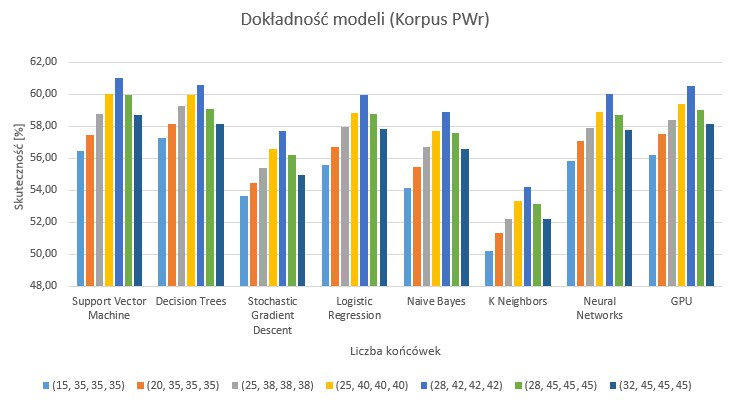
\includegraphics[width=\linewidth]{korpuspwrwykres}
	\label{Rysunek}
	\caption{Skuteczność modeli -- Korpus PWr}
\end{figure}

\begin{figure}[!htbp]
	\centering
	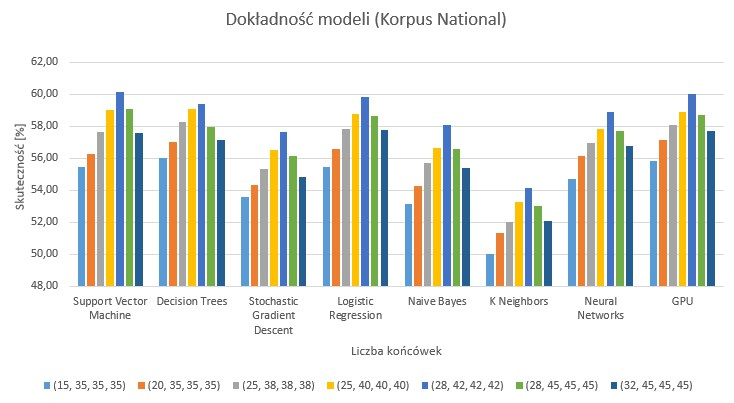
\includegraphics[width=\linewidth]{korpusnationalwykres}
	\label{Rysunek}
	\caption{Skuteczność modeli -- Korpus National}
\end{figure}

